\chapter{NUMERICAL SOLUTION}
\label{chap:numerical}

In this chapter, the mathematical details involved in the numerical solution of the previously described equations are presented.
It is assumed that this model is run in conjunction with a model describing the growth of kelp over its life cycle, which calls this light model periodically to update the light field.

\section{Super-Individuals}

The algorithm described in this chapter has two components.
First, a probabilistic description of the kelp is generated at each point in a discrete spatial grid.
Second, optical properties of the resulting kelp-water medium are derived, and the light field is calculated.
The first component is described here.

\subsection{Frond Length Distribution}

Rather than model each kelp frond, a subset of the population, called super-individuals, are modeled explicitly, and are considered to represent many identical individuals, as in \citep{scheffer_super-individuals_1994}.
Specifically, at each depth $k$, there are $n$ super-individuals, indexed by $i$.
Super-individual $i$ has a frond area $A_{ki}$ and represents $n_{ki}$ individual fronds.

From \eqref{eqn:length-from-area}, the frond length of the super-individual is $l_{ki} = \sqrt{2A_{ki}f_r}$.
Given the super-individual data, we calculate the mean $\mu$ and standard deviation $\sigma$ frond
lengths using the formulas:
\begin{equation*}
  \mu_k = \frac{\ds \sum_{i=1}^N l_{ki}}{\ds \sum_{i=1}^N n_{ki}},
\end{equation*}
\begin{equation*}
  \sigma_k = \frac{\ds \sum_{i=1}^N \left( l_{ki} - \mu_k \right)^2}{\ds \sum_{i=1}^N n_{ki}}.
\end{equation*}
We then assume that frond lengths are normally distributed in each depth layer
with mean $\mu_k$ and standard deviation $\sigma_k$.

\section{Discrete Grid}
The following is a description of the spatial-angular grid used in the numerical implementation of this model.
It is assumed that all simulated quantities are constant over the interior of a grid cell.
Other legitimate choices of grids exists; this one was chosen for its relative simplicity.

The domain of the radiative transfer equation is embedded in five dimensions: three spatial ($x$, $y$, and $z$) and two angular (azimuthal $\theta$ and polar $\phi$).
The number of grid cells in each dimension are denoted by $n_x$, $n_y$, $n_z$,
$n_\theta$, and $n_\phi$, with uniform spacings $dx$, $dy$, $dz$, $d\theta$, and
$d\phi$ between adjacent grid points.

The following indices are assigned to each dimension:
\begin{align*}
  x &\to i \\
  y &\to j \\
  z &\to k \\
  \theta &\to l \\
  \phi &\to m
\end{align*}

It is convenient, however, to use a single index $p$ to refer to directions $\vec{\omega}$ rather than referring to $\theta$ and $\phi$ separately.
Then, the center of a generic grid cell will be denoted as
$(x_i, y_j, z_k, \vec{\omega}_p)$, and the boundaries between adjacent grid cells
will be referred to as \textit{edges}.
One-indexing is employed throughout this document.

\begin{figure}[H]
  \centering
  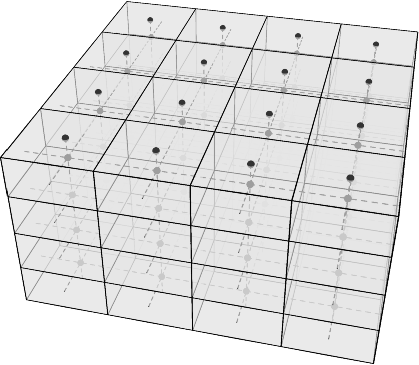
\includegraphics[width=8cm]{spatialgrid.pdf}
  \caption{Spatial grid}
  \label{fig:spatial_grid}
\end{figure}

Each spatial grid cell is the Cartesian product of $x$, $y$, and $z$ intervals of width $dx$, $dy$, and $dz$ respectively.
The three-dimensional interval centered at $(x_i, y_j, z_k)$ is denoted $X_{ijk}$, and has volume $\abs{X_{ijk}}=dx\,dy\,dz$.
Also, note that no grid center is located on the plane $z=0$; the surface radiance boundary condition is treated separately.

\begin{figure}[H]
  \centering
  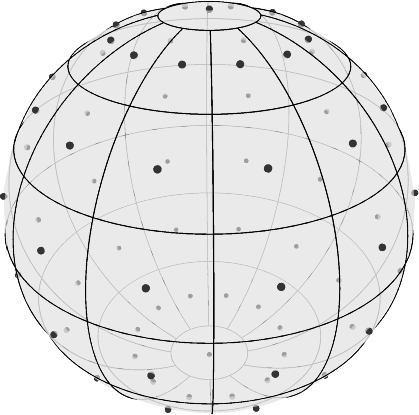
\includegraphics[width=8cm]{angulargrid.pdf}
  \caption{Angular grid at each point in space}
  \label{fig:angular_grid}
\end{figure}

As shown in Figure \ref{fig:angular_grid}, $\phi=0$ and $\phi=\pi$, called
the north ($+z$) and south ($-z$) poles respectively, are treated separately from other angular grid cells.
A generic interior angular grid cell centered at $\vec{\omega}_p$ is the Cartesian product of an azimuthal interval of width $d\theta$ and a polar interval of width $d\theta$.
However, two pole cells are the Cartesian product of a polar interval of width $d\phi/2$ and the full azimuthal domain, $[0, 2\pi)$.

With this configuration, the total number of angles considered is $\nomega = n_\theta(n_\phi-2)+2$.
Then, cells are indexed by $p=1,\ldots,n_{\vec{\omega}}$ and are ordered such that
$p=1$ and $p=n_{\vec{\omega}}$ refer to the north and south poles respectively,
$p\leq\nomega/2$ refers to the northern hemisphere, and $p>\nomega/2$ refers to the southern hemisphere.
Further, the symbol $\Omega_p$ is used to refer to the two dimension angular interval centered at $\omega_p$.
The solid angle subtended by $\Omega_p$ is denoted $\abs{\Omega_p}$.
Refer to Appendix \ref{chap:grid_details} for a more rigorous discussion of the discrete spatial-angular grid.

\section{Quadrature Rules}
Since it is assumed that all quantities are constant within a spatial-angular grid cell,
the midpoint rule is employed for both spatial and angular integration.
Presented here is a basic derivation of the formulas for integration in the spatial-angular grid.
Further details are found in Appendix \ref{chap:ray_tracing}.

Define the \textit{spatial characteristic function}
\begin{equation*}
  \mathcal{X}^X_{ijk}(\vec{x}) = \begin{cases}
    1, & \vec{x} \in X_{ijk} \\
    0, & \mbox{otherwise}
  \end{cases}
\end{equation*}
and the \textit{angular characteristic function}
\begin{equation*}
  \mathcal{X}^\Omega_p(\vec{\omega}) = \begin{cases}
    1, & \vec{\omega} \in \Omega_p \\
    0, & \mbox{otherwise}.
  \end{cases}
\end{equation*}

\subsection{Spatial Quadrature}
The double integral of a function $f(\vec{x})$ over a depth layer $k$ is approximated as
\begin{align*}
  \int_\xmin^\xmax\int_\ymin^\ymax f(x, y, z_k)\, dy\, dx &\approx \int_\xmin^\xmax \int_\ymin^\ymax \sum_{i=1}^{n_x}\sum_{j=1}^{n_y} \mathcal{X}^X_{ijk}(x,y,z_k) f(x_i, y_j, z_k)\, dy\, dx \\
  &= \sum_{i=1}^{n_x}\sum_{j=1}^{n_y} f(x_i, y_j, z_k) \int_\xmin^\xmax \int_\ymin^\ymax \mathcal{X}^X_{ijk}(x,y,z_k) \, dy\, dx \\
  &= \sum_{i=1}^{n_x}\sum_{j=1}^{n_y} \abs{X_{ijk}} f(x_i, y_j, z_k) \\
  &= dx\, dy\, dx\, \sum_{i=1}^{n_x}\sum_{j=1}^{n_y} f(x_i, y_j, z_k).
\end{align*}
The path integral of $f(\vec{x})$ over a path $\vec{l}(s)$ from $s=0$ to $s=\tilde{s}$ is
\begin{align*}
  \int_0^{\tilde{s}} f(\vec{l}(s))\, ds &= \sum_{ijk} f(x_i, y_j, z_k)\, ds_{ijk},
\end{align*}
where $ds_{ijk}$ is the total path distance of $\vec{l}(s)$ through $X_{ijk}$.
Full details of the path integral algorithm for the case of straight line paths are found in Appendix \ref{chap:ray_tracing}.

\subsection{Angular Quadrature}
Then, the integral of a function $f(\vec{\omega})$ is approximated as
\begin{align*}
  \int_{4\pi} f(\vec{\omega})\, d\vec{\omega} &\approx \int_{4\pi} \sum_{p=1}^\nomega f(\vec{\omega}_p) \mathcal{X}^\Omega_p(\vec{\omega})\, d\vec{\omega} \\
  &= \sum_{p=1}^\nomega f(\vec{\omega}_p) \int_{4\pi} \mathcal{X}^\Omega_p(\vec{\omega})\, d\vec{\omega} \\
  &= \sum_{p=1}^\nomega f(\vec{\omega}_p) \int_{\Omega_p} d\vec{\omega} \\
  &= \sum_{p=1}^\nomega f(\vec{\omega}_p) \abs{\Omega_p}.
\end{align*}

\section{Numerical Asymptotics}
Presented here are details of the evaluation of the asymptotic approximations \eqref{eqn:asymptotics_soln_0} and \eqref{eqn:asymptotics_soln_n} to the raditiave transfer equation \eqref{eqn:rte}.

\subsection{Scattering Integral}

Specifically, the amount of light scattered between angular grid cells is found by integrating $\beta$ as follows.
Consider two angular grid cells, $\Omega$ and $\Omega'$.
The average probability density of scattering from $\vec{\omega} \in \Omega$ to $\vec{\omega}' \in \Omega'$ (or vice versa) is
\begin{equation*}
  \beta_{pp'} = \frac{1}{\abs{\Omega}\abs{\Omega'}} \int_\Omega\int_{\Omega'}\beta(\vec{\omega}\cdot\vec{\omega}')\, d\vec{\omega'}\, d\vec{\omega}
\end{equation*}

Denote the radiance at $(x_i, y_j, z_k, \vec{\omega}_p)$ by $L_{ijkp}$.
% TODO: Be more careful here.
Then, the total radiance scattered into $\Omega_p$ from $\Omega_{p'}$ is
\begin{align*}
  \int_{\Omega}\int_{\Omega'}\beta(\vec{\omega} \cdot \vec{\omega}')L(\vec{x},\vec{\omega}')\, d\vec{\omega}'\, d\vec{\omega}
  &= L_{ijkp'} \int_\Omega\int_{\Omega_{p'}} \beta(\vec{\omega} \cdot \vec{\omega}')\, d\vec{\omega}'\, d\vec{\omega} \\
  &= \beta_{pp'}\abs{\Omega}\abs{\Omega'}L_{ijkp'}.
\end{align*}
Hence, the average radiance scattered is $\beta_{pp'}\abs{\Omega'}L_{ijkp'}.$

\subsection{Ray Integral}
Given a position $\vec{x}$ and direction $\vec{\omega}$, a path through the discrete grid can be constructed as described in Appendix \ref{chap:ray_tracing}, from which we can extract piecewise constant variations of the path absorption coefficient, $\tilde{a}(s)$ and the effective source, $g_n(s)$ from Section \ref{sec:asymptotic_sol}.
Then, we proceed as follows.

* Here are the equations for calculating the double integral over ray paths
required for the asymptotics. It will hopefully make more sense once I add words
to accompany the symbols.

Let
\begin{align*}
  g_n(s) &= \sum_{i=1}^{N-1}g_{ni}\mathcal{X}_i(s) \\
  \tilde{a}(s) &= \sum_{i=1}^{N-1}\tilde{a}_{i}\mathcal{X}_i(s) \\
\end{align*}
and
\begin{equation*}
  \mathcal{X}_i(s) = \begin{cases}
    1, & a_I \leq s < s_{i+1} \\
    0, & \mbox{otherwise}
    \end{cases}
\end{equation*}

and $\left\{s_i\right\}_{i=1}^N$ is increasing.

Let $ds_i = s_{i+1} - s_i$.

Let $\hat{i}(s) = \min\left\{ i \in \{1,\ldots,N\} : s_i>s \right\}$.
Let $\tilde{d}(s) = s_{\hat{i}(s)}-s$.

We have $s_1 = 0$ and $s_N = \tilde{s}$.


\begin{align*}
  u_n(\tilde{s}) &= \int_0^{\tilde{s}}g_n(s')\exp\left( -\int_{s''}^{s'}\tilde{a}(s'')\,ds'' \right)\, ds' \\
  &= \int_0^{s_N} \sum_{i=1}^{N-1}g_{ni}\mathcal{X}_i(s') \exp\left( -\int_{s''}^{s'}\sum_{j=1}^{N-1}\tilde{a}_{j}\mathcal{X}_j(s'')\,ds'' \right)\, ds' \\
  &= \sum_{i=1}^{N-1}g_{ni}\int_0^{s_N} \mathcal{X}_i(s') \exp\left( -\sum_{j=1}^{N-1}\tilde{a}_{j}\int_{s''}^{s'}\mathcal{X}_j(s'')\,ds'' \right)\, ds' \\
  &= \sum_{i=1}^{N-1}g_{ni}\int_{s_i}^{s_{i+1}}  \exp\left(-\tilde{a}_{\hat{i}(s')-1}\tilde{d}(s') -\sum_{j=\hat{i}(s')}^{N-1}\tilde{a}_{j}ds_j\right)\, ds' \\
  &= \sum_{i=1}^{N-1}g_{ni}\int_{s_i}^{s_{i+1}}  \exp\left(-\tilde{a}_{i}(s_{i+1}-s') -\sum_{j=i+1}^{N-1}\tilde{a}_{j}ds_j\right)\, ds'
\end{align*}

Let
\begin{equation*}
  b_i = -\tilde{a}_{i}s_{i+1} - \sum_{j=i+1}^{N-1}\tilde{a}_{j}ds_j.
\end{equation*}

Then,
\begin{align*}
  u_n(\tilde{s}) &= \sum_{i=1}^{N-1}g_{ni}\int_{s_i}^{s_{i+1}}  \exp\left(\tilde{a}_{i}s' + b_i\right)\, ds' \\
                 &= \sum_{i=1}^{N-1}g_{ni}e^{b_i}\int_{s_i}^{s_{i+1}}  \exp\left(\tilde{a}_{i}s'\right) ds'
\end{align*}

Let
\begin{align*}
  d_i &= \int_{s_i}^{s_{i+1}}  \exp\left(\tilde{a}_{i}s'\right)\, ds' \\
    &= \begin{cases}
    ds_i, & \tilde{a} = 0 \\
      \left( \exp(\tilde{a}_i s_{i+1}) - \exp(\tilde{a}_i s_i) \right)/\tilde{a}_i, & \mbox{otherwise}
    \end{cases}
\end{align*}

Then,
\begin{equation*}
  u_n(\tilde{s}) = \sum_{i=1}^{N-1} g_{ni}d_i e^{b_i}
\end{equation*}

\section{Finite Difference}

We now discuss the discretization of derivatives on the spatial grid.

\subsection{Discretization}

For the spatial interior of the domain, we use the second order central difference formula (CD2) to approximate the derivatives, which is
\begin{equation*}
    \tag{CD2}
    f'(x) = \frac{f(x+dx)-f(x-dx)}{2dx} + \mathcal{O}(dx^3).
\end{equation*}

When applying the PDE on the upper or lower boundary, we use the forward and backward difference (FD2 and BD2) formulas respectively.
Omitting $\mathcal{O}(dx^3)$, we have
\begin{equation*}
    \tag{FD2}
    \label{eq:FD2}
    f'(x) = \frac{-3f(x)+4f(x+dx)-f(x+2dx)}{2dx}
\end{equation*}
\begin{equation*}
    \tag{BD2}
    \label{eq:BD2}
    f'(x) = \frac{3f(x)-4f(x-dx)+f(x-2dx)}{2dx}
\end{equation*}

For the upper and lower boundaries, we need an asymmetric finite difference
method.
In general, the Taylor Series of a function $f$ about $x$ is
\begin{equation*}
  f'(x+\varepsilon) = \sum_{n=1}^\infty \frac{f^{(n)}(x)}{n!} \varepsilon^n \\
\end{equation*}

Truncating after the first few terms, we have
\begin{equation}
  \label{eqn:afd1}
  f'(x+\varepsilon)  = f(x) + f'(x)\varepsilon + \frac{f''(x)}{2}\varepsilon^2 + \mathcal{O}(\varepsilon^3)
\end{equation}

Similarly, replacing $\varepsilon$ with $-\varepsilon/2$ we have
\begin{equation}
  \label{eqn:afd2}
  f'(x-\frac{\varepsilon}{2}) = f(x) - \frac{f'(x)\varepsilon}{2} + \frac{f''(x)\varepsilon^2}{8} + \mathcal{O}(\varepsilon^3).
\end{equation}

Rearranging \eqref{eqn:afd1} produces
\begin{equation}
  \label{eqn:afd3}
  f''(x)\varepsilon^2 = 2f(x+\varepsilon) - 2f(x) - 2f'(x)\varepsilon + \mathcal{O}(\varepsilon^3)
\end{equation}

Combining \eqref{eqn:afd2} with \eqref{eqn:afd3} gives
\begin{align*}
  \varepsilon f'(x) &= 2f(x) - 2f(x-\frac{\varepsilon}{2}) + f''(x)\frac{\varepsilon^2}{8} + \mathcal{O}(\varepsilon^3) \\
                    &= 2f(x) - 2f(x-\frac{\varepsilon}{2}) + \frac{f(x+\varepsilon)}{4} - \frac{f(x)}{4} - \frac{f'(x)\varepsilon}{4} + \mathcal{O}(\varepsilon^3) \\
                    &= \frac{4}{5}\left( 2f(x)-2f(x-\frac{\varepsilon}{2}) + \frac{f(x+\varepsilon)}{4} - \frac{f(x)}{4} \right) + \mathcal{O}(\varepsilon^3)
\end{align*}

Then, dividing by $\varepsilon$ gives
\begin{equation*}
  f'(x) = \frac{-8f(x-\frac{\varepsilon}{2}) + 7f(x) + f(x+\varepsilon)}{5\varepsilon} + \mathcal{O}(\varepsilon^2)
\end{equation*}

Similarly, substituting $\varepsilon \to -\varepsilon$, we have 
\begin{equation*}
  f'(x) = \frac{- f(x-\varepsilon) - 7f(x) + 8f(x+\frac{\varepsilon}{2})}{5\varepsilon} + \mathcal{O}(\varepsilon^2)
\end{equation*}


\subsection{Difference Equation}

%TODO: Periodic $x,y$

In general, we have

\begin{equation*}
  \vec{\omega} \cdot \nabla L_p = -(a+b) L_p + \sum_{p'=1}^{n_{\vec{\omega}}} \beta_{pp'}L_{p'}.
\end{equation*}

Then,
\begin{equation*}
  \vec{\omega} \cdot \nabla L_p + (a+b(1-\beta_{pp'}))L_p - \sum_{p'=1}^{n_{\vec{\omega}}} \beta_{pp'} L_{p'} = 0
\end{equation*}

Interior:
\begin{equation*}
  \begin{aligned}
    0 &= \frac{L_{i+1,jkp}-L_{i-1,jkp}}{2dx}\sin\hat{\phi}_p\cos\hat{\theta}_p \\
    &+ \frac{L_{i,j+1,kp}-L_{i,j-1,kp}}{2dy}\sin\hat{\phi}_p\sin\hat{\theta}_p \\
    &+ \frac{L_{ij,k+1,p}-L_{ij,k-1,p}}{2dz}\cos\hat{\phi}_p \\
    &+ (a_{ijk}+b(1-\beta_{pp'}))L_{ijkp}  - \sum_{p'=1}^{n_{\vec{\omega}}} \beta_{pp'} L_{ijkp'}
  \end{aligned}
\end{equation*}

Surface downwelling (BC):
\begin{equation*}
  \begin{aligned}
    0 &= \frac{L_{i+1,jkp}-L_{i-1,jkp}}{2dx}\sin\hat{\phi}_p\cos\hat{\theta}_p \\
    &+ \frac{L_{i,j+1,kp}-L_{i,j-1,kp}}{2dy}\sin\hat{\phi}_p\sin\hat{\theta}_p \\
    &+ \frac{-8f_p + 7L_{ijkp} + L_{ij,k+1,p}}{5dz}\cos\hat{\phi}_p \\
    &+ (a_{ijk}+b(1-\beta_{pp'}))L_{ijkp} \\
    &- \sum_{p'=1}^{n_{\vec{\omega}}} \beta_{pp'} L_{ijkp'}.
  \end{aligned}
\end{equation*}

Combining $L_{ijkp}$ terms on the left and moving the boundary condition to the
right gives

\begin{equation*}
  \begin{aligned}
    &\frac{L_{i+1,jkp}-L_{i-1,jkp}}{2dx}\sin\hat{\phi}_p\cos\hat{\theta}_p \\
    + &\frac{L_{i,j+1,kp}-L_{i,j-1,kp}}{2dy}\sin\hat{\phi}_p\sin\hat{\theta}_p \\
    + &\frac{L_{ij,k+1,p}}{5dz}\cos\hat{\phi}_p \\
    + &(a_{ijk}+b(1-\beta_{pp'}) + \frac{7}{5dz} \cos\hat{\phi}_p)L_{ijkp} \\
    - &\sum_{p'=1}^{n_{\vec{\omega}}} \beta_{pp'} L_{ijkp'} = \frac{8f_p}{5dz} \cos\hat{\phi}_p.
  \end{aligned}
\end{equation*}

Likewise for the bottom boundary condition, we have

\begin{equation*}
  \begin{aligned}
    0 &= \frac{L_{i+1,jkp}-L_{i-1,jkp}}{2dx}\sin\hat{\phi}_p\cos\hat{\theta}_p \\
    &+ \frac{L_{i,j+1,kp}-L_{i,j-1,kp}}{2dy}\sin\hat{\phi}_p\sin\hat{\theta}_p \\
    &- \frac{L_{ij,k-1,p}}{5dz}\cos\hat{\phi}_p \\
    &+ (a_{ijk}+b(1-\beta_{pp'}) - \frac{7}{5dz}\cos\hat{\phi}_p)L_{ijkp} \\
    &- \sum_{p'=1}^{n_{\vec{\omega}}} \beta_{pp'} L_{ijkp'}.
  \end{aligned}
\end{equation*}

Now, for upwelling light at the first depth layer (non-BC), we apply FD2.
\begin{equation*}
  \begin{aligned}
    0 &= \frac{L_{i+1,jkp}-L_{i-1,jkp}}{2dx}\sin\hat{\phi}_p\cos\hat{\theta}_p \\
    &+ \frac{L_{i,j+1,kp}-L_{i,j-1,kp}}{2dy}\sin\hat{\phi}_p\sin\hat{\theta}_p \\
    &+ \frac{-3L_{ijkp} + 4L_{ij,k+1,p} - L_{ij,k+2,p}}{2dz}\cos\hat{\phi}_p \\
    &+ (a_{ijk}+b(1-\beta_{pp'}))L_{ijkp} \\
    &- \sum_{p'=1}^{n_{\vec{\omega}}} \beta_{pp'} L_{ijkp'}.
  \end{aligned}
\end{equation*}

Grouping $L_{ijkp}$ terms gives
\begin{equation*}
  \begin{aligned}
    0 &= \frac{L_{i+1,jkp}-L_{i-1,jkp}}{2dx}\sin\hat{\phi}_p\cos\hat{\theta}_p \\
    &+ \frac{L_{i,j+1,kp}-L_{i,j-1,kp}}{2dy}\sin\hat{\phi}_p\sin\hat{\theta}_p \\
    &+ \frac{4L_{ij,k+1,p} - L_{ij,k+2,p}}{2dz}\cos\hat{\phi}_p \\
    &+ \left(a_{ijk}+b(1-\beta_{pp'}) - 3\frac{\cos\hat\phi_p}{2dz} \right)L_{ijkp} \\
    &- \sum_{p'=1}^{n_{\vec{\omega}}} \beta_{pp'} L_{ijkp'}.
  \end{aligned}
\end{equation*}

Similarly, for downwelling light at the lowest depth layer, we have
\begin{equation*}
  \begin{aligned}
    0 &= \frac{L_{i+1,jkp}-L_{i-1,jkp}}{2dx}\sin\hat{\phi}_p\cos\hat{\theta}_p \\
    &+ \frac{L_{i,j+1,kp}-L_{i,j-1,kp}}{2dy}\sin\hat{\phi}_p\sin\hat{\theta}_p \\
    &+ \frac{-4L_{ij,k-1,p} + L_{ij,k-2,p}}{2dz}\cos\hat{\phi}_p \\
    &+ \left(a_{ijk}+b(1-\beta_{pp'}) + 3\frac{\cos\hat\phi_p}{2dz} \right)L_{ijkp} \\
    &- \sum_{p'=1}^{n_{\vec{\omega}}} \beta_{pp'} L_{ijkp'}
  \end{aligned}
\end{equation*}

\subsection{Structure of Linear System}

%TODO: This
Describe layout of matrix.

\begin{table}[H]
  \centering
  \begin{tabular}{p{\linewidth/3}p{\linewidth/3}p{\linewidth/3}}
    \toprule
    \textbf{Derivative case} & \textbf{\# nonzero/row} & \textbf{\# of rows} \\
    \midrule
    interior & $\nomega+6$ & $n_xn_y(n_z-2)\nomega$ \\
    surface downwelling & $\nomega+5$ & $n_xn_y\nomega/2$ \\
    bottom upwelling & $\nomega+5$ & $n_xn_y\nomega/2$ \\
    surface upwelling & $\nomega+6$ & $n_xn_y\nomega/2$ \\
    bottom downwelling & $\nomega+6$ & $n_xn_y\nomega/2$ \\
  \end{tabular}
  \caption{Breakdown of nonzero matrix elements by derivative case}
\end{table}

Number of rows/columns: $n_xn_yn_zn_{\vec{\omega}}$

Number of nonzero RHS entries: $n_xn_yn_z/2$

Total number of nonzero matrix entries: $n_xn_yn_{\vec{\omega}} \left[n_z(n_{\vec{\omega}}+6)-1 \right]$

\subsection{GMRES}
% TODO: Fill this in
GMRES is a Krylov Subspace method. These work like this. Here's what's special
about GMRES. Advantages. Drawbacks. Not practical for running in SINMOD.

\subsection{Perceived Irradiance}
\label{sec:perceived_irrad}

The average irradiance experienced by a kelp frond in depth layer $k$ is
\newcommand{\Iperk}{\tilde{I}_k}
\begin{equation*}
   \Iperk = \frac{\sum_{ij}P_{ijk}I_{ijk}}{\sum_{ij}P_{ijk}}.
\end{equation*}

The irradiance perceived by the kelp is expected to be slightly lower than the average irradiance,
\begin{equation*}
  \bar{I}_k = \frac{\sum_{ij}I_{ijk}}{n_x n_y}
\end{equation*}
since the kelp is more densely located at the center of the domain where the light field is reduced,
whereas the simple average is influenced by regions of higher irradiance at the edges of the domain where kelp is not present.
